\subsection{Ecuación de recurrencia de primer orden}

\begin{frame}
\frametitle{\secname}
\framesubtitle{\subsecname}

\begin{block}{Solución general a la ecuación de recurrencia}
	Considere la ecuación de recurrencia \[ S_{n+1}=aS_{n}+c,\qquad\forall n\in\mathds{N}. \]
	\begin{description}
		\item[Primer caso] Si $a=1$, entonces $S_{n}= S_{0}+nc$, $\forall n\in \mathds{N}$.
		\item[Segundo caso] Si $a\neq1$, entonces $S_{n}=a^{n}\left[S_{0}-\frac{c}{1-a}\right]+\frac{c}{1-a}$, $\forall n\in\mathds{N}$.
	\end{description}
	\end{block}
\end{frame}

\subsubsection{Torre de Hanói}

\begin{frame}
%\frametitle{\secname}
%\framesubtitle{\subsecname}
\begin{minipage}{0.45\paperwidth}
Considere la ecuación de recurrencia \[ S_{n}=2S_{n-1}+1,\quad\forall n\geq2, \] donde $n$ denota el número de discos y $S_{n}$ es el mínimo número de movimientos necesario para transportar los $n$ discos desde una aguja a otra.
\end{minipage}
\hfill
\begin{minipage}{0.45\paperwidth}
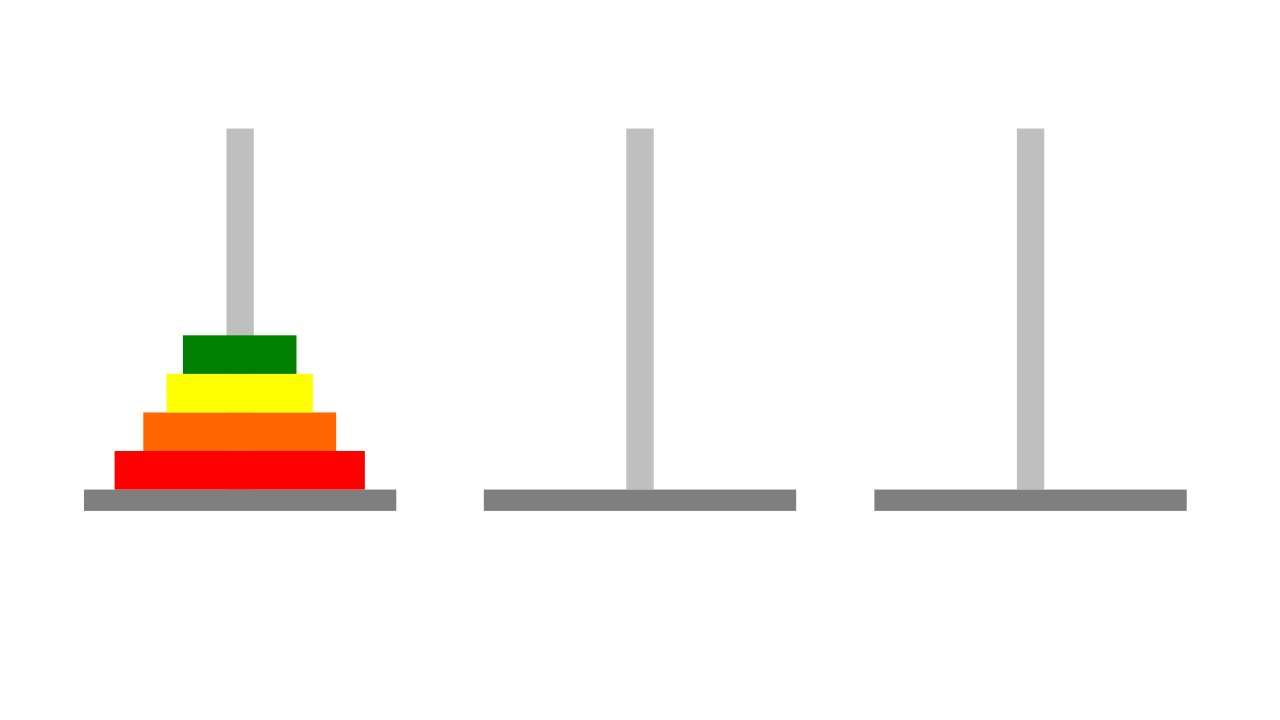
\includegraphics[width=0.4\paperwidth]{torre.jpg}
\end{minipage}
\end{frame}

\begin{frame}
%\frametitle{\secname}
%\framesubtitle{\subsecname}
\frametitle{Ecuación de recurrencia de segundo orden}

\begin{theorem}
$S_n = A(r_1)^n + B(r_2)^n$ si $r_1 \neq r_2$, siempre que $\Delta\neq0$.
\end{theorem}

\begin{theorem}
$S_n = A(r)^n + Bn(r)^n$ si $r_1 = r_2 = r$, siempre que $\Delta=0$.
\end{theorem}
\end{frame}

\begin{frame}
%\frametitle{\secname}
%\framesubtitle{\subsecname}
\frametitle{Un modelo de la cunicultura}
Considere la ecuación de recurrencia \[ F_{n}=F_{n-1}+F_{n-2},\quad\forall n\geq2, \] llamada \textbf{ecuación de Fibonacci}.

\

\begin{minipage}{0.45\paperwidth}
Fibonacci partía de ciertas hipótesis, a saber:
	\begin{itemize}
		\item Los conejos viven eternamente.
		\item Cada mes, un par de adultos de distinto sexo da lugar a un nuevo par de conejos de distinto sexo.
		\item Cada conejo se hace adulto a los dos meses de vida, momento en el que comienza a tener descendencia.
	\end{itemize}
\end{minipage}
\hfill
\begin{minipage}{0.45\paperwidth}
	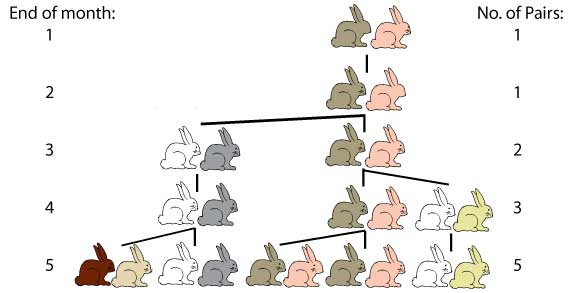
\includegraphics[width=0.4\paperwidth]{conejos.jpg}
\end{minipage}

\end{frame}